\documentclass[a4paper, papersize, titlepage]{jsarticle}
\usepackage[]{multicol} % 途中からtwocolumun \begin{multicols}{n}
\usepackage[dvipdfmx]{graphicx}

% for \mathbb{}, \begin{cases}
\usepackage{amsmath, amssymb}
\usepackage{type1cm} 
\usepackage{url}
\usepackage{comment}
\usepackage{mathtools} % for \coloneqq
\usepackage{eqnarray} % 連続するn式
\usepackage{here}


\usepackage{listings,jlisting} % 日本語のコメントアウトをする場合jlistingが必要
% ここからソースコードの表示に関する設定
\lstset{
  basicstyle={\ttfamily},
  identifierstyle={\small},
  commentstyle={\smallitshape},
  keywordstyle={\small\bfseries},
  ndkeywordstyle={\small},
  stringstyle={\small\ttfamily},
  frame={tb},
  breaklines=true,
  columns=[l]{fullflexible},
  numbers=left,
  xrightmargin=0zw,
  xleftmargin=3zw,
  numberstyle={\scriptsize},
  stepnumber=1,
  numbersep=1zw,
  lineskip=-0.5ex
}
% ここまでソースコードの表示に関する設定
% \begin{lstlisting}[caption=hoge,label=fuga] を用いる
% キャプション名「ソースコードn」を「プログラムn」に変えるには,\begin{document}の前に\renewcommand{\lstlistingname}{プログラム}
% https://qiita.com/ta_b0_/items/2619d5927492edbb5b03

% for hyperref
\usepackage[dvipdfmx, bookmarkstype=toc, colorlinks=false, pdfborder={0 0 0}, bookmarks=true, bookmarksnumbered=true]{hyperref}
\usepackage{pxjahyper}

\def\bm#1{\mbox{\boldmath $#1$}} % for bm (vector)

%%%%%%%%%%%%%%%%%%%%%%%%%%%%%%%%%%%%%%%%%%%%%%%%%%%%%%%%%%%%%%%%%%%%%%%%%%%%%%%%

\title{高度情報演習2C \\
【前半】テーマ1(真鍋)1回目レポート \\
~\\
仮説「ターゲットまでの距離が遠い場合,\\
ポインティングが完了するまでの時間は長い」\\
の真偽の検証
}
\author{片岡 凪 \thanks{芝浦工業大学 工学部 情報工学科 3年 学籍番号AL18036}}
\date{提出日 2020年10月25日}

\begin{document}

\maketitle
\setcounter{tocdepth}{3}
\tableofcontents

\newpage
% \begin{abstract}
% hoge
% \end{abstract}

\begin{multicols}{2}

\begin{comment}
【講義資料の要点】
・お題「ターゲットまでの距離が遠い場合,ポインティングが完了するまでの時間は長い」の検証
・何を計測するか
・リハーサル(動作,トリガー,期待する結果か,時間,辛いか,修正,指示)
・1人5分以内
・3人
・試行順番はランダム 順序効果を打ち消す
・統一したところ
・練習は事前に1分(統一)
・指示はいつ誰がどのように
・被験者はどのような人か
・プライバシー保護
・中止したければ中止できることを伝える
・バイアスをかけない(何を意図した研究なのか)
・2種類の実験を混ぜない(だけど,別のパラメータと比較できるとよい?)

【分析・解析】
・傾向,発見
・外れ値はないか
・失敗試行は除外
・散布図,ヒストグラム
・誤差,個人差
・計測値と母集団の違いを考慮し検定
・母集団が,正規分布で分散も等しい,と仮定し,t検定
・Excelで検定,作図
・特定の実験協力者に限るのか一般に言えるのか注意
・散布図の一次近似

【ポイント】
•なぜその実験を行うのか!!
•どのような実験を行ったのか
•どのような結果が得られたのか
•結果をどのように分析したのか
•分析の結果,あなたは何を主張するのか!!
•2つ以上のグラフ(計測値,分析結果等)

・複数の選択肢を挙げ,なぜそれを選んだか
→順番,失敗の対応,形状,大きさ,グラフ,試行回数
・棒グラフには標準偏差
・まだ解明できていない点を述べる
・Unityとは何か,を説明する

【アイディア】
・円→点の精度を得たかった
・距離の精度を得たい場合,バウムクーヘンの形にするべき?
・休日の夜に揃える
・ディスプレイのサイズ
・各々が使い慣れているマウスと速度
・低速度ポインタと高速度ポインタが存在

【言いたい事】
・仮説の証明
・計測値の平均の増加
・母集団の平均の差

【次の課題】
・色を変えると命中度は変わるか → 色相,コントラスト
・従来手法 提案手法
・適当な論文を読んで,課題を実装

\end{comment}

%%%%%%%%%%%%%%%%%%%%%%%%%%%%%%%%%%%%%%%%%%%%%%%%%%%%%%%%%%%%%%%%%%%%%%%%%%%%%%%%

\section{実験目的}
本実験では,コンピュータの入力装置のひとつである光学マウスを用いて,講義で指定された仮説「ターゲットまでの距離が遠い場合,ポインティングが完了するまでの時間は長い」が正しいかどうかの検証を行う.
ここで,仮説に用いた各用語は以下のように定量的に定義する.

\begin{itemize}
\item ターゲット
\begin{itemize}
\item ポインティングデバイス\footnote{2.1で詳しく述べる}の主用途であるコンピュータ上のGUI\footnote{Graphical User Interfaceの略称.マウスカーソルなどを用いて視覚的にコンピュータを操作する機能体系を指す.}の一種,ボタンを想定した,クリック時の有効範囲が点対称な図形
\item マウスカーソルの初期座標とは異なる座標に点対称の対称の中心が位置する,クリックしようとする対象
\end{itemize}

\item ターゲットまでの距離が遠い
\begin{itemize}
\item マウスカーソルの初期座標$(x_0, y_0)$とターゲットの重心の座標$(x_1, y_1)$とのユークリッド距離 $\sqrt{(x_0 - x_1)^2 + (y_0 - y_1)^2}$ が大きい
\end{itemize}

\item ポインティングが完了するまでの時間は長い
\begin{itemize}
\item マウスカーソルが初期座標から動き始める直前の時刻から,ターゲットをクリックするまでの時刻までの時刻の差
\end{itemize}

\item ターゲットまでの距離が遠い場合,ポインティングが完了するまでの時間は長い
\begin{itemize}
\item ターゲットまでの距離とポインティングが完了するまでの時間に正の相関がある
\end{itemize}
\end{itemize}
%%%%%%%%%%%%%%%%%%%%%%%%%%%%%%%%%%%%%%%%%%%%%%%%%%%%%%%%%%%%%%%%%%%%%%%%%%%%%%%%

% \section{関連研究}

% \subsection{Ninja cursors}

% \subsection{foo}

%%%%%%%%%%%%%%%%%%%%%%%%%%%%%%%%%%%%%%%%%%%%%%%%%%%%%%%%%%%%%%%%%%%%%%%%%%%%%%%%

% \section{提案手法}
\section{原理}
\subsection{ポインティングデバイス}
ポインティングデバイスとは,コンピュータの入力装置であり,ディスプレイ上の位置情報と操作に必要なコマンドを送るための周辺機器の総称である.GUI環境で,カーソルを動かす,アイコンをクリックするなどの操作を行う~\cite{pointing_device_bib}.本実験で扱うポインティングデバイスには,呼びかけた全ての被験者が使い慣れていると述べた光学マウスを選択した.

カーソルの位置情報とクリックボタンが押下される情報はそれぞれ独立に取得される.本実験では,クリックボタンが押下するタイミングで位置情報や時刻などのデータを収集する機能を実装する.

また,光学マウスを動かしたときの位置情報の変位量はコンピュータ側で調節が可能である.本実験では,被験者が普段扱い慣れている速度に設定した.

%%%%%%%%%%%%%%%%%%%%%%%%%%%%%%%%%%%%%%%%%%%%%%%%%%%%%%%%%%%%%%%%%%%%%%%%%%%%%%%%

\section{実験器具}

以下の実験器具を用いて実験を行った.

\begin{itemize}
\item コンピュータ
\begin{itemize}
\item 後述のUnityが軽快に動作するもの
\item 本実験では,Panasonic製のCF-SZ5PDYVSで統一した
\begin{itemize}
\item CPU : i5-6300U
\item メモリ : LPDDR3 8GB
\item ストレージ : SATA SSD
\item OS : Windows 10 Pro
\end{itemize}
\end{itemize}

\item ディスプレイ
\begin{itemize}
\item 本実験では,BENQ製のGL2460で統一した
\begin{itemize}
\item 24インチ
\item 解像度 1920x1080
\item リフレッシュレート 60Hz
\end{itemize}
\end{itemize}

\item ポインティングデバイス
\begin{itemize}
\item 光学マウス
\item 被験者が使い慣れている被験者の所有物を使用
\begin{itemize}
\item 全ての被験者が,扱い慣れていない同一のデバイスを用いた場合よりも,被験者間の諸データの差が小さくなると判断したため.本実験では行わなかったが,同一のデバイスを用いた実験を検討する必要性も少なくない.
\end{itemize}
\end{itemize}

\item Unity
\begin{itemize}
\item Version 2019.4.11f1 Personal
\item 主にゲームを開発するためのプラットフォーム~\cite{unity_bib}
\item ゲームの開発に必要なポインティングデバイスの入力情報を取得,操作する機能をもつため,本実験での利用に適していると考える
\end{itemize}

\item Unity
\begin{itemize}
\item Version 2019.4.11f1 Personal
\item 主にゲームを開発するためのプラットフォーム~\cite{unity_bib}
\item ゲームの開発に必要なポインティングデバイスの入力情報を取得,操作する機能をもつため,本実験での利用に適していると考える
\item プログラミング言語 \verb|C#| 7.3 を包含し,これと併用してソフトウェア各機能を実装する
\end{itemize}

\item Microsoft Visual Studio Community 2019
\begin{itemize}
\item Version 4.8.04084
\item \verb|C#|を記述するための統合開発環境
\end{itemize}

\item Microsoft Excel
\begin{itemize}
\item Version 2009 (Build 13231.20418)
\item ポインティングデバイスから取得したデータの作図や検定に用いる
\end{itemize}
\end{itemize}

% \subsection{アプリケーション}

%%%%%%%%%%%%%%%%%%%%%%%%%%%%%%%%%%%%%%%%%%%%%%%%%%%%%%%%%%%%%%%%%%%%%%%%%%%%%%%%

\section{実験方法}

\subsection{ソフトウェアの実装}

\subsubsection{ターゲットの外見,形状}
本実験で実装したターゲットは,ポインティングデバイスの主用途であるGUIの一種,ボタンを想定し,図~\ref{target_looks}に示すように,ポインティングデバイスの最大径の3倍の直径をもつ正円とした.ターゲットの大きさは,図~\ref{browser_button},~\ref{latex_button}に示すように,ウェブブラウザやウェブサービスのボタンを参考にした.これらの図からわかるように,図~\ref{target_looks}の正円より直径が大きいボタンは,何度も押下する重要なボタンであると考えられ,押下しやすいように横幅が長く設計されており,またその長さはツールによってばらつきが大きい.より一般的な形状を扱うため,ターゲットの形状は正円あるいは正方形が適当だと考えた.

後述の理由で図\ref{target_looks}のように外側のターゲットを円環状に配置するのが妥当だと考えたため,ターゲットを正方形にした場合,外側の正方形をどのように回転させたとしても,マウスカーソルの初期座標と正方形との対称性が悪い,あるいはボタンとしては一般的でない,正方形の各辺がディスプレイの縁と平行とならない回転角になってしまう.そのため,本実験では正方形ではなく正円を採用した.

また,ターゲットのデザインは,図\ref{target_looks}のように,ビデオゲームやアナログゲームなどでよく見受けられる紅白の縞模様とした.このデザインにすることで,ユーザーにターゲットがクリック対象であると認識させやすくなり,ボタンと近い心理状況に持ち込めるものと考える.なお,同様の理由で,マウスカーソルの初期座標にも全く同じ形状,サイズ,デザインのターゲットを配置した.

 さらに,ゲームのタイムアタックのシーンでよく見受けられるターゲットのデザインであるため,本実験で測定したい「ポインティングが完了するまでの時間」がユーザの可能な限り短くなるような効果が得られると期待する.

% \renewcommand{\figurename}{図4-}
\begin{figure}[H]
 \centering
   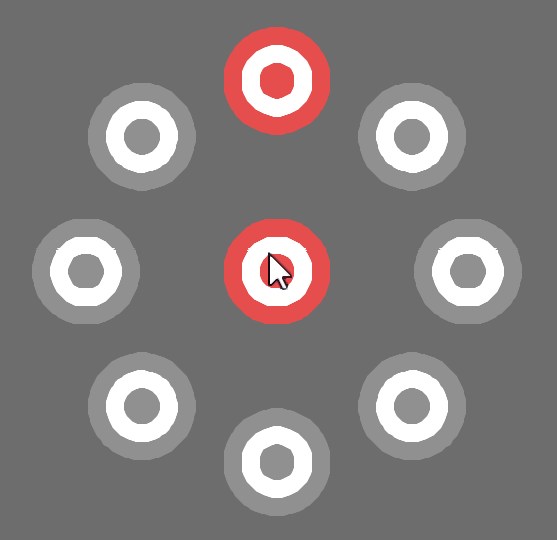
\includegraphics[width=65mm]{target_looks.png}
 \caption{マウスポインタと比較したターゲットの外見,形状}
 \label{target_looks}
\end{figure}
\noindent


% \renewcommand{\figurename}{図4-}
\begin{figure}[H]
 \centering
   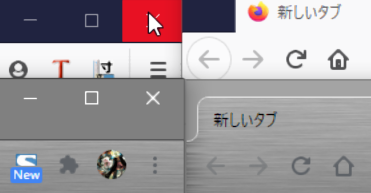
\includegraphics[width=65mm]{browser_button.png}
 \caption{ウェブブラウザFirefox(上)とGoogle Chrome(下)のボタンの大きさ}
 \label{browser_button}
\end{figure}
\noindent


% \renewcommand{\figurename}{latex_button.png}
\begin{figure}[H]
 \centering
   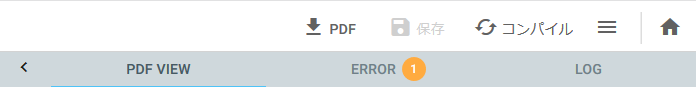
\includegraphics[width=65mm]{latex_button.png}
 \caption{ウェブサービス Cloud LaTeXのボタンの大きさ}
 \label{latex_button}
\end{figure}
\noindent

%%%%%%%%%%%%%%%%%%%%

\subsubsection{ターゲットの配置}
マウスカーソルの初期座標の位置を含む中心のターゲットの中心座標はウィンドウの中心に固定し,その周辺にターゲットの座標を配置した.赤色のターゲットが初期座標のターゲットの次にクリックさせるターゲットである.

ここで,ポインティング時にマウスを動かす方向によって「ポインティングが完了するまでの時間」が変化してしまうものと考え,図~\ref{target_pos}のように,外側のターゲットは$360[^\circ] / 8 = 45[^\circ]$ の間隔で均等に配置した.外側のターゲットは常に1つを赤色に,それ以外を灰色にし,どの順番でどの位置が赤色になるかはソフトウェアの実行時にランダムで設定する.

図~\ref{target_looks}, 図~\ref{target_pos}の違いからわかるように,「ターゲットまでの距離」は等間隔で4段階用意した.異なる位置の外側の赤いターゲットを8回クリックする度に,この間隔を変更する.どの順番でどの間隔になるかは,ソフトウェアの実行時にランダムで設定する.

外側の赤いターゲットの位置は,上に述べたことから本実験では$8\times4 = 32$箇所の定位置に出現するが,今後の検定のため,理想をいえば無作為に抽出した位置にするのが適当であると考える.しかし,本実験では講義時間の長さや被験者の実験による疲労を鑑み,得られるデータが少ないため,無作為抽出を行ってしまうとデータの分散が大きくなり,今後の検定で良い結果が得られないと考える.代わりにターゲットの出現座標を32箇所に揃え,分散の小さいデータを得るのが適当であると考える.

得られるデータが多い際には,

% \renewcommand{\figurename}{図4-}
\begin{figure}[H]
 \centering
   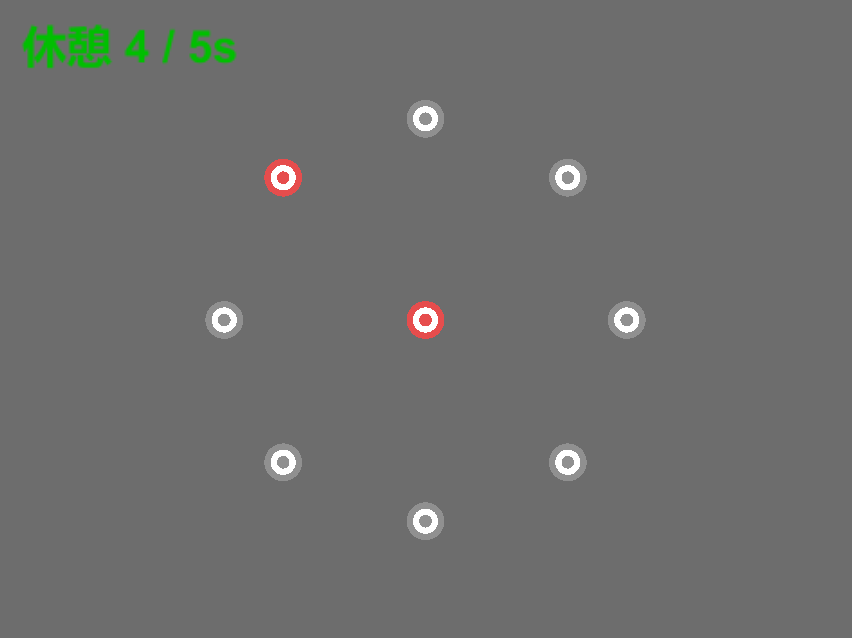
\includegraphics[width=65mm]{target_pos.png}
 \caption{ウィンドウ上の32か箇所にランダムに配置される外側の赤いターゲット}
 \label{target_pos}
\end{figure}
\noindent

% \subsubsection{ターゲットの衝突判定}
% \subsubsection{試行回数}


\subsubsection{休憩時間のカウント}
実験は,中心のターゲットをクリックし,外側の赤いターゲットをクリックする1セットの操作を32回繰り返す.このとき,被験者に常に同じ条件,すなわち同じ疲労度で操作を行わせるために,各セットで5秒間の休憩を挟ませた.

被験者に休憩時間であることを伝えるために,図~\ref{target_pos}, ~\ref{breaktime}のように画面左上に休憩時間のカウントを表示した.5秒間は緑の字でカウントされ,0秒になると赤字になる.また,3秒から0秒にかけて,時報のサウンドエフェクトを鳴らした.被験者の心理状況になるべく影響を与えないようにするため,被験者に聞きなじみのある音を選定した\footnote{OtoLogicのZihou01-1.mp3を利用した\cite{zihou_bib}}


\subsubsection{データの取得}
データは検定と検定以外の傾向の発見のため,外側の赤いターゲットのクリック時に,上述の4段階の距離情報,8段階の角度情報と,ターゲットの中心とクリック座標からの距離(4段階に正規化した),「ポインティングが完了するまでの時間」の4つを記録した.「ポインティングが完了するまでの時間」の取得のため,中心のターゲットのクリック時の時刻情報を取得するように実装した.

外側の赤いターゲットをクリックしようとして灰色の背景をクリックしてしまった場合もターゲットの位置は変わるように設定し,記録した距離から判別して外れ値として排除した.なぜなら,ターゲットが変わらずに1セットで3回以上クリックしてしまうケースは,2回でクリックが完了する期待するデータとは「ポインティングが完了するまでの時間」の条件が満たされている,揃っているとは言い難いためである.

なお,クリックが行われたことを被験者にわかりやすく伝え,直感的な操作を可能にするために,クリック時にはクリック音\footnote{OtoLogicのPC-Mouse01-1.mp3を利用した~\cite{click_bib}}が鳴るように設定した.


% \renewcommand{\figurename}{図4-}
\begin{figure}[H]
 \centering
   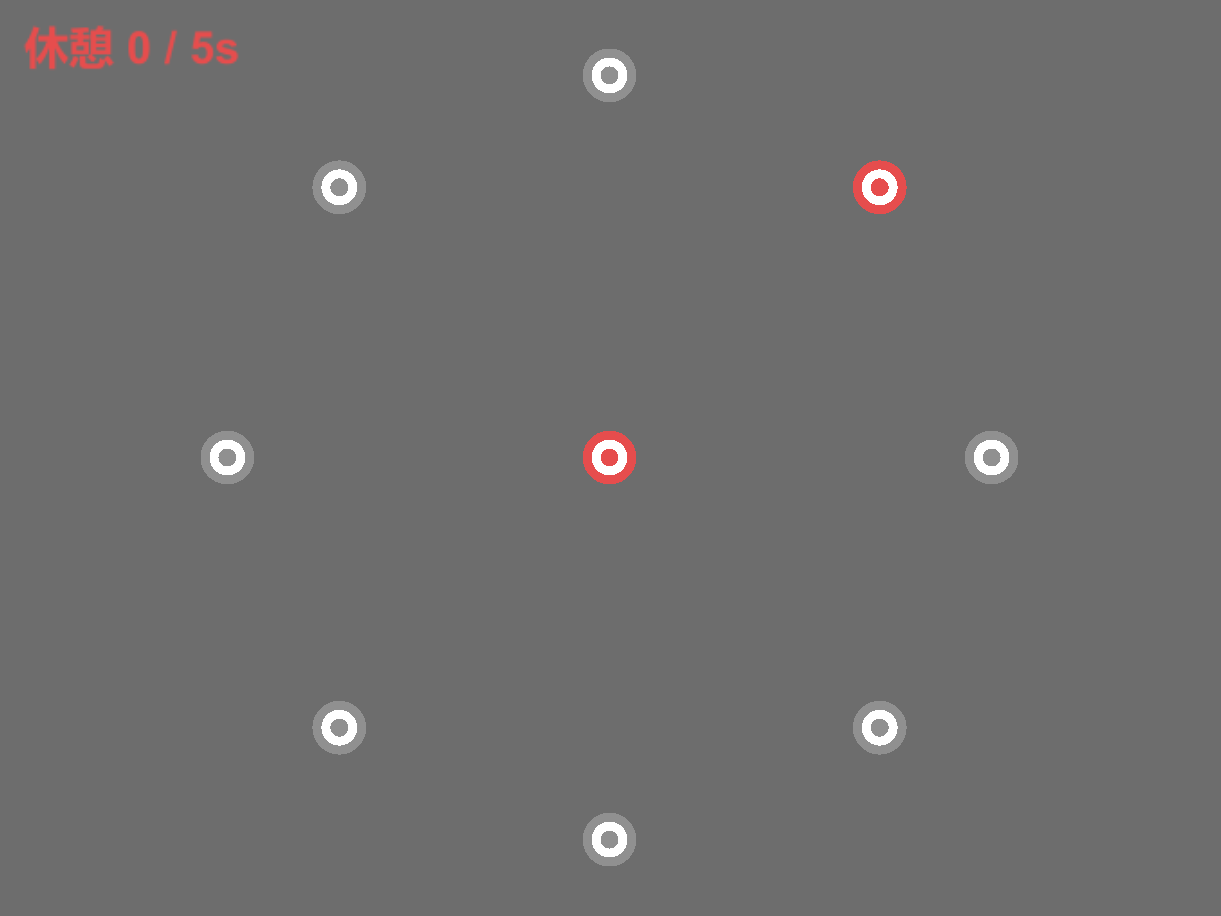
\includegraphics[width=65mm]{breaktime.png}
 \caption{時刻0sで色が変わる休憩時間のカウント}
 \label{breaktime}
\end{figure}
\noindent

\subsubsection{画面のサイズ}
実験はUnity上で行った.各実験で画面のサイズが揃うよう,図~\ref{exe_window}の赤二重線で示した場所に位置するMaximize on window機能を用いてUnityのウィンドウを最大化して実験を行った.

% \renewcommand{\figurename}{図4-}
\begin{figure}[H]
 \centering
   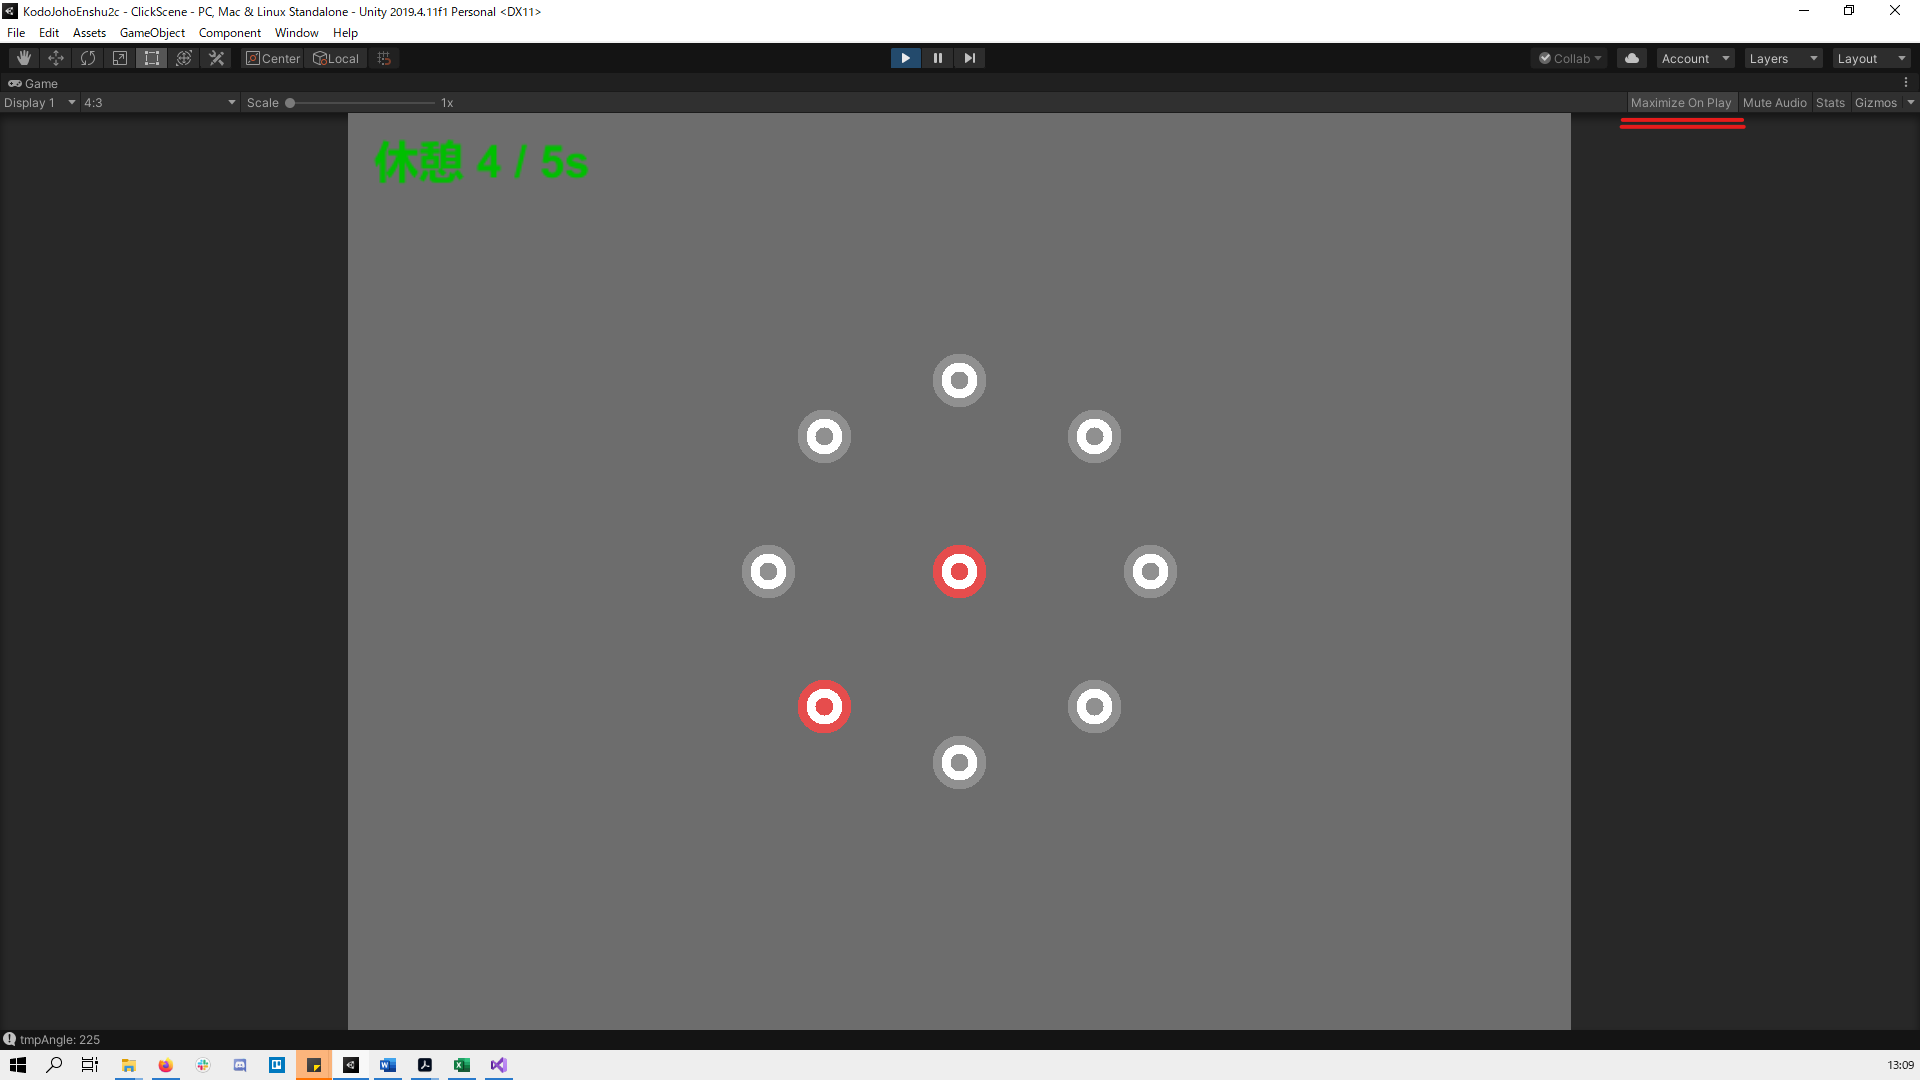
\includegraphics[width=65mm]{exe_window.png}
 \caption{ディスプレイ全体から見た実験時のイメージ}
 \label{exe_window}
\end{figure}
\noindent

\subsection{データの分析}



\subsection{被験者の選定}
本実験では,情報科学を専攻する男子学生1名,情報科学系統の企業に勤める男性1名,同じく情報科学系統の企業に勤める女性1名に協力を仰いだ.3名とも情報科学に携わる20代の若者であり,ポインティングディバイスの操作速度は近しいものと考えられる.

より確かな仮説の実証を行うためには,より多くの職業,年齢層,人数のデータを得る必要がある.

\subsection{被験者への説明}

以下の項目を,Unityの画面を見せながら被験者に説明した.

\begin{itemize}
\item 実験途中であっても,被験者の意向でいつでも実験を中止できる
\item 個人を特定するデータは記録も公開もされない
\item 被験者の年齢と職業をレポートに掲載する
\item データは講義課題のみに使用する
\item 説明の後に厳密な1分間の練習時間を設ける
\item 画面中心のターゲットをクリックした後に外側の赤いターゲットをクリックする操作を,ソフトウェアが停止するまで繰り返す
\item 外側の赤いターゲットをクリックした後,5秒間の休憩時間がカウントされるので,それまでにカーソルを画面中心に戻し,カウントが0になったら画面中心のターゲットをクリックする
\item カウントダウンはあくまで目安なので,多少前後しても構わない
\item 可能な限り速くマウスを動かし,クリックを行う
\item 座標の精度は考えず,ターゲットのどこか一部をクリックすればよい
\item 外側の赤いターゲットの位置はランダムに変化するので注意する
% \item ターゲット付近に当たると音が鳴るが,クリック位置がターゲットと離れすぎて音が鳴らない場合は再度同じターゲットのクリックを試みる
\item 最初は自分のタイミングで,中心のターゲットからスタートする
\item (実験終了後)質問や感想がないか
\begin{itemize}
\item 正常でない心理状況でなかったかを確認する
\item 被験者の意見から何かしらの発見がある可能性がある
\end{itemize}
\end{itemize}

%%%%%%%%%%%%%%%%%%%%%%%%%%%%%%%%%%%%%%%%%%%%%%%%%%%%%%%%%%%%%%%%%%%%%%%%%%%%%%%%

\section{実験結果}
\subsection{実験中の発見}
\subsubsection{座標の補正方法の変容}
「ターゲットの距離が遠い」ほど,感覚でターゲットの方向にマウスを大きく動かし,行き過ぎてしまった分を補正するという傾向が強く見受けられた.一方,「ターゲットの距離が近い」ほど,マウスポインターを減速させつつ座標を補正しようとする傾向が強く見受けられた.

今後の課題として,ターゲットの距離でどちらの補正方法を取ることが多いのか,また他の補正方法が存在し得るかのデータを取得し,本実験で得るようなデータと比較・分析を行うことで,より確かな仮説の立証が可能であると考える.

\subsubsection{始点と終点がともに視界に入るか否か}
被験者からのヒアリングで,「ターゲットの距離が遠い」と2点のターゲットを同時に視界に入れるのが難しく,どちらを見ていたら良いのかがわからなくなった,という意見が得られた.この状況とそうでない状況では,「ポインティングが完了するまでの時間」に有意な差が見られるものと考える.

今後の課題として,ターゲットの距離がどれほど大きくなれば2点のターゲットを同時に視界に入れるのが難しくなるのかを検証し,本実験で得るようなデータと比較・分析を行うことで,より確かな仮説の立証が可能であると考える.

\subsection{取得したデータ}
3名の被験者から取得したデータ,4段階の距離情報,8段階の角度情報と,ターゲットの中心とクリック座標からの距離(4段階に正規化した),「ポインティングが完了するまでの時間」は,次の表~\ref{table}の通りになった.

\renewcommand{\figurename}{表}
\begin{figure}[H]
 \centering
 \caption{取得したデータの表}
   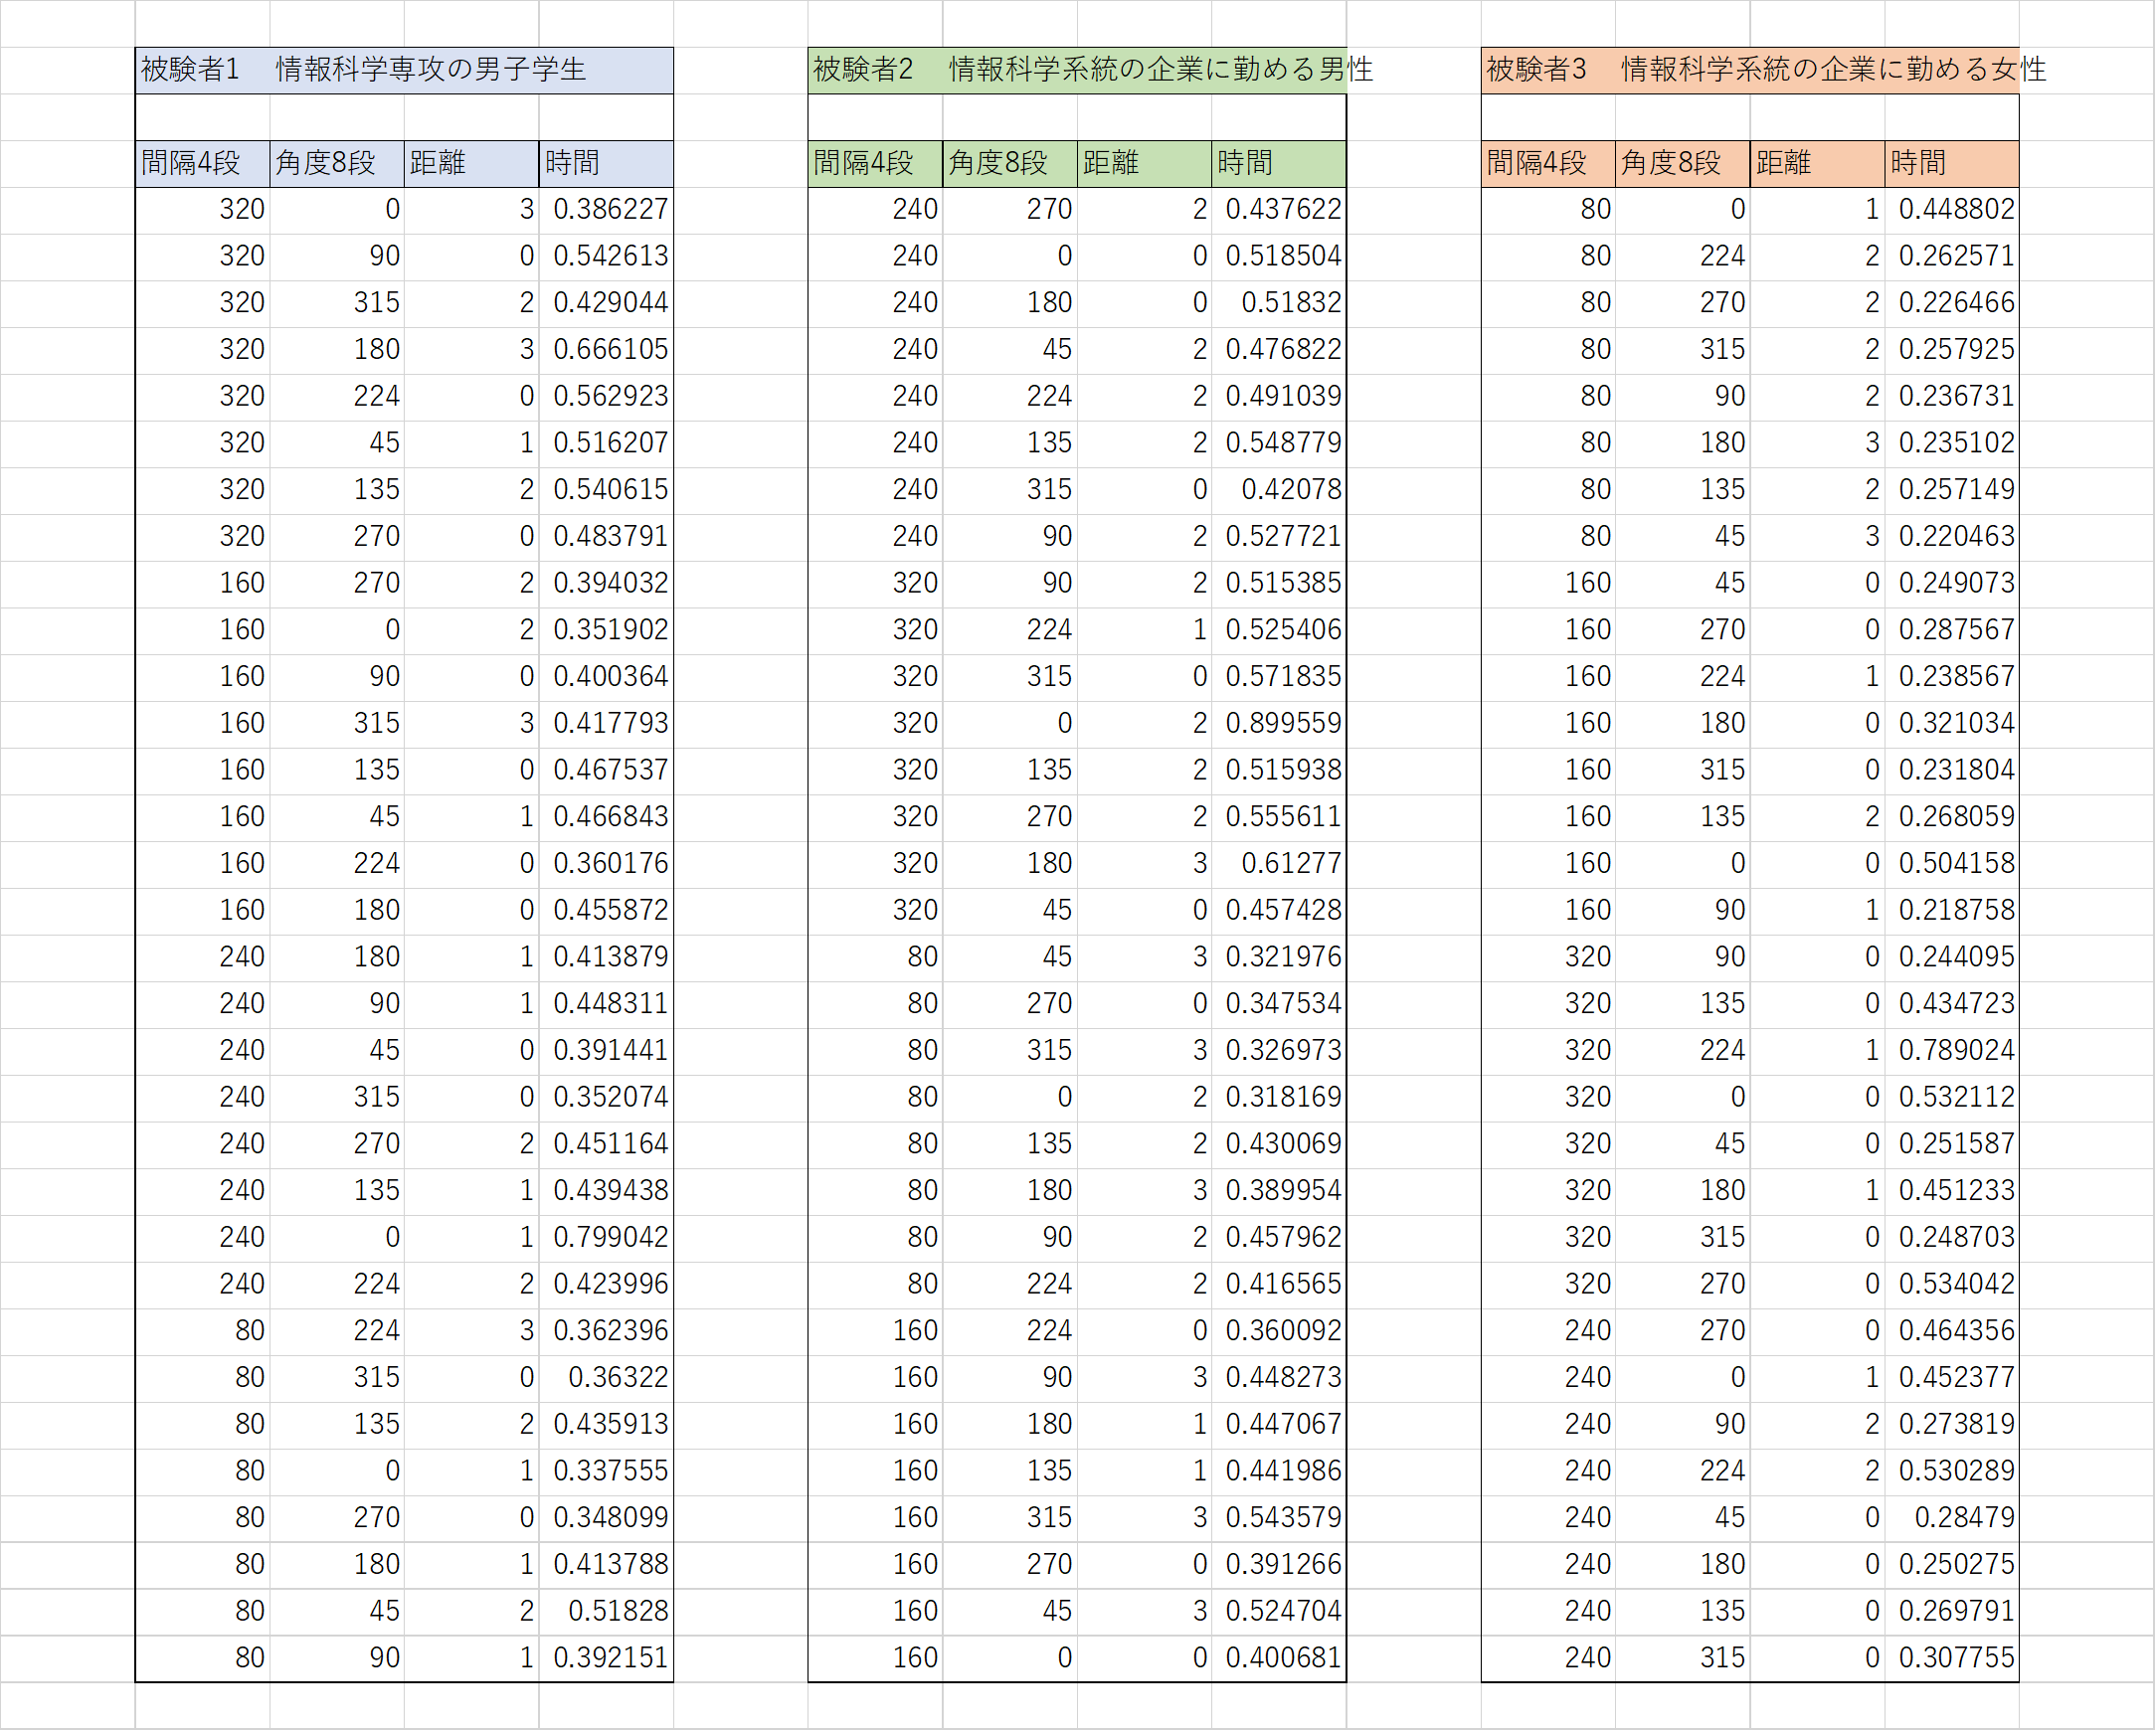
\includegraphics[width=75mm]{table.png}
 \label{table}
\end{figure}
\noindent

\subsection{データの分析結果}
以下のデータ分析は,表~\ref{table}の距離のスコアが0のもの,すなわちターゲット上を正しくクリックできなかったデータは全て外れ値を見なし,除外して行った.

\subsubsection{散布図と近似曲線}
図~\ref{plot}のようにデータを散布図に取り,被験者ごとに一次式で近似すると,どの近似曲線も傾きが正となった.
% 軸の説明

このことから,これらの被験者のデータからは仮説「ターゲットまでの距離が遠い場合,ポインティングが完了するまでの時間は長い」が正しいといえる.

\renewcommand{\figurename}{図}
\begin{figure}[H]
 \centering
   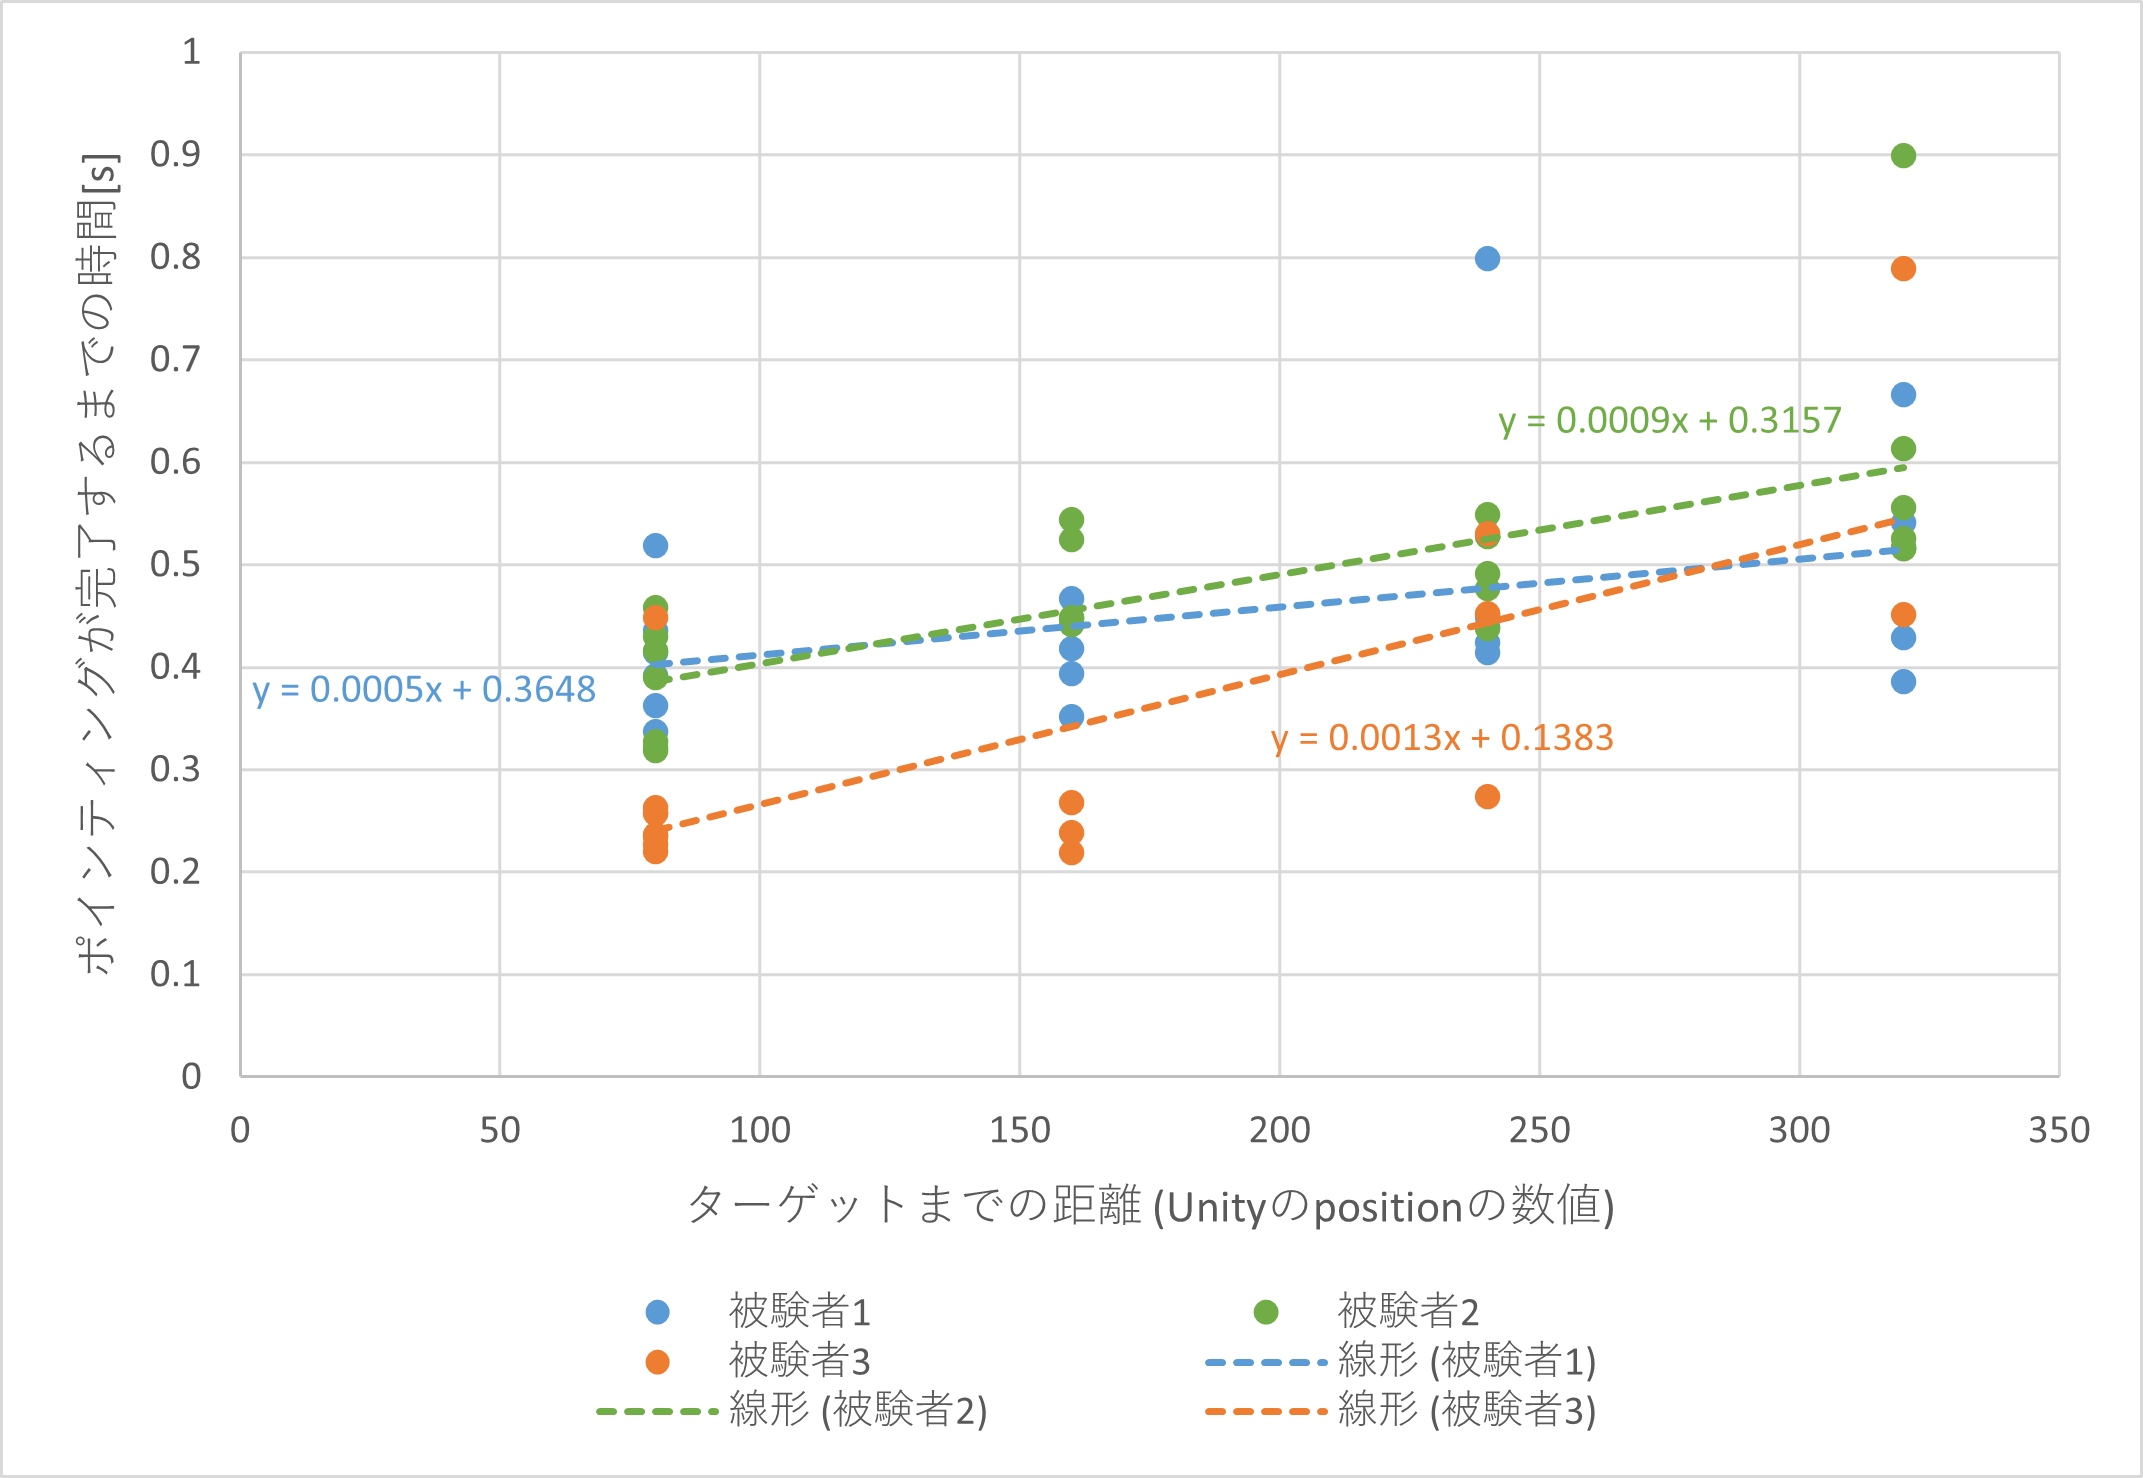
\includegraphics[width=65mm]{plot.png}
 \caption{被験者ごとに色分けしたデータの散布図と近似曲線}
 \label{plot}
\end{figure}
\noindent

\subsubsection{箱ひげ図}
得られたデータのうち,全被験者の「ターゲットまでの距離」ごとの外れ値の数が最も少なかった「ターゲットまでの距離」は,80であった.
この最も外れ値の少ない「ターゲットまでの距離」80という同一の条件の下,「ポインティングが完了するまでの時間」をについて箱ひげ図を作図した結果,図~\ref{hige}のようになった.
データ数は少ないが,最小値,最大値と各四分位数およそ均等に配置されていそうなことから,抽出した標本が正規分布に従っていそうである.より正規分布に近い分布であれば,今後のt検定の精度が高いといえる.

% \renewcommand{\figurename}{図}
\begin{figure}[H]
 \centering
   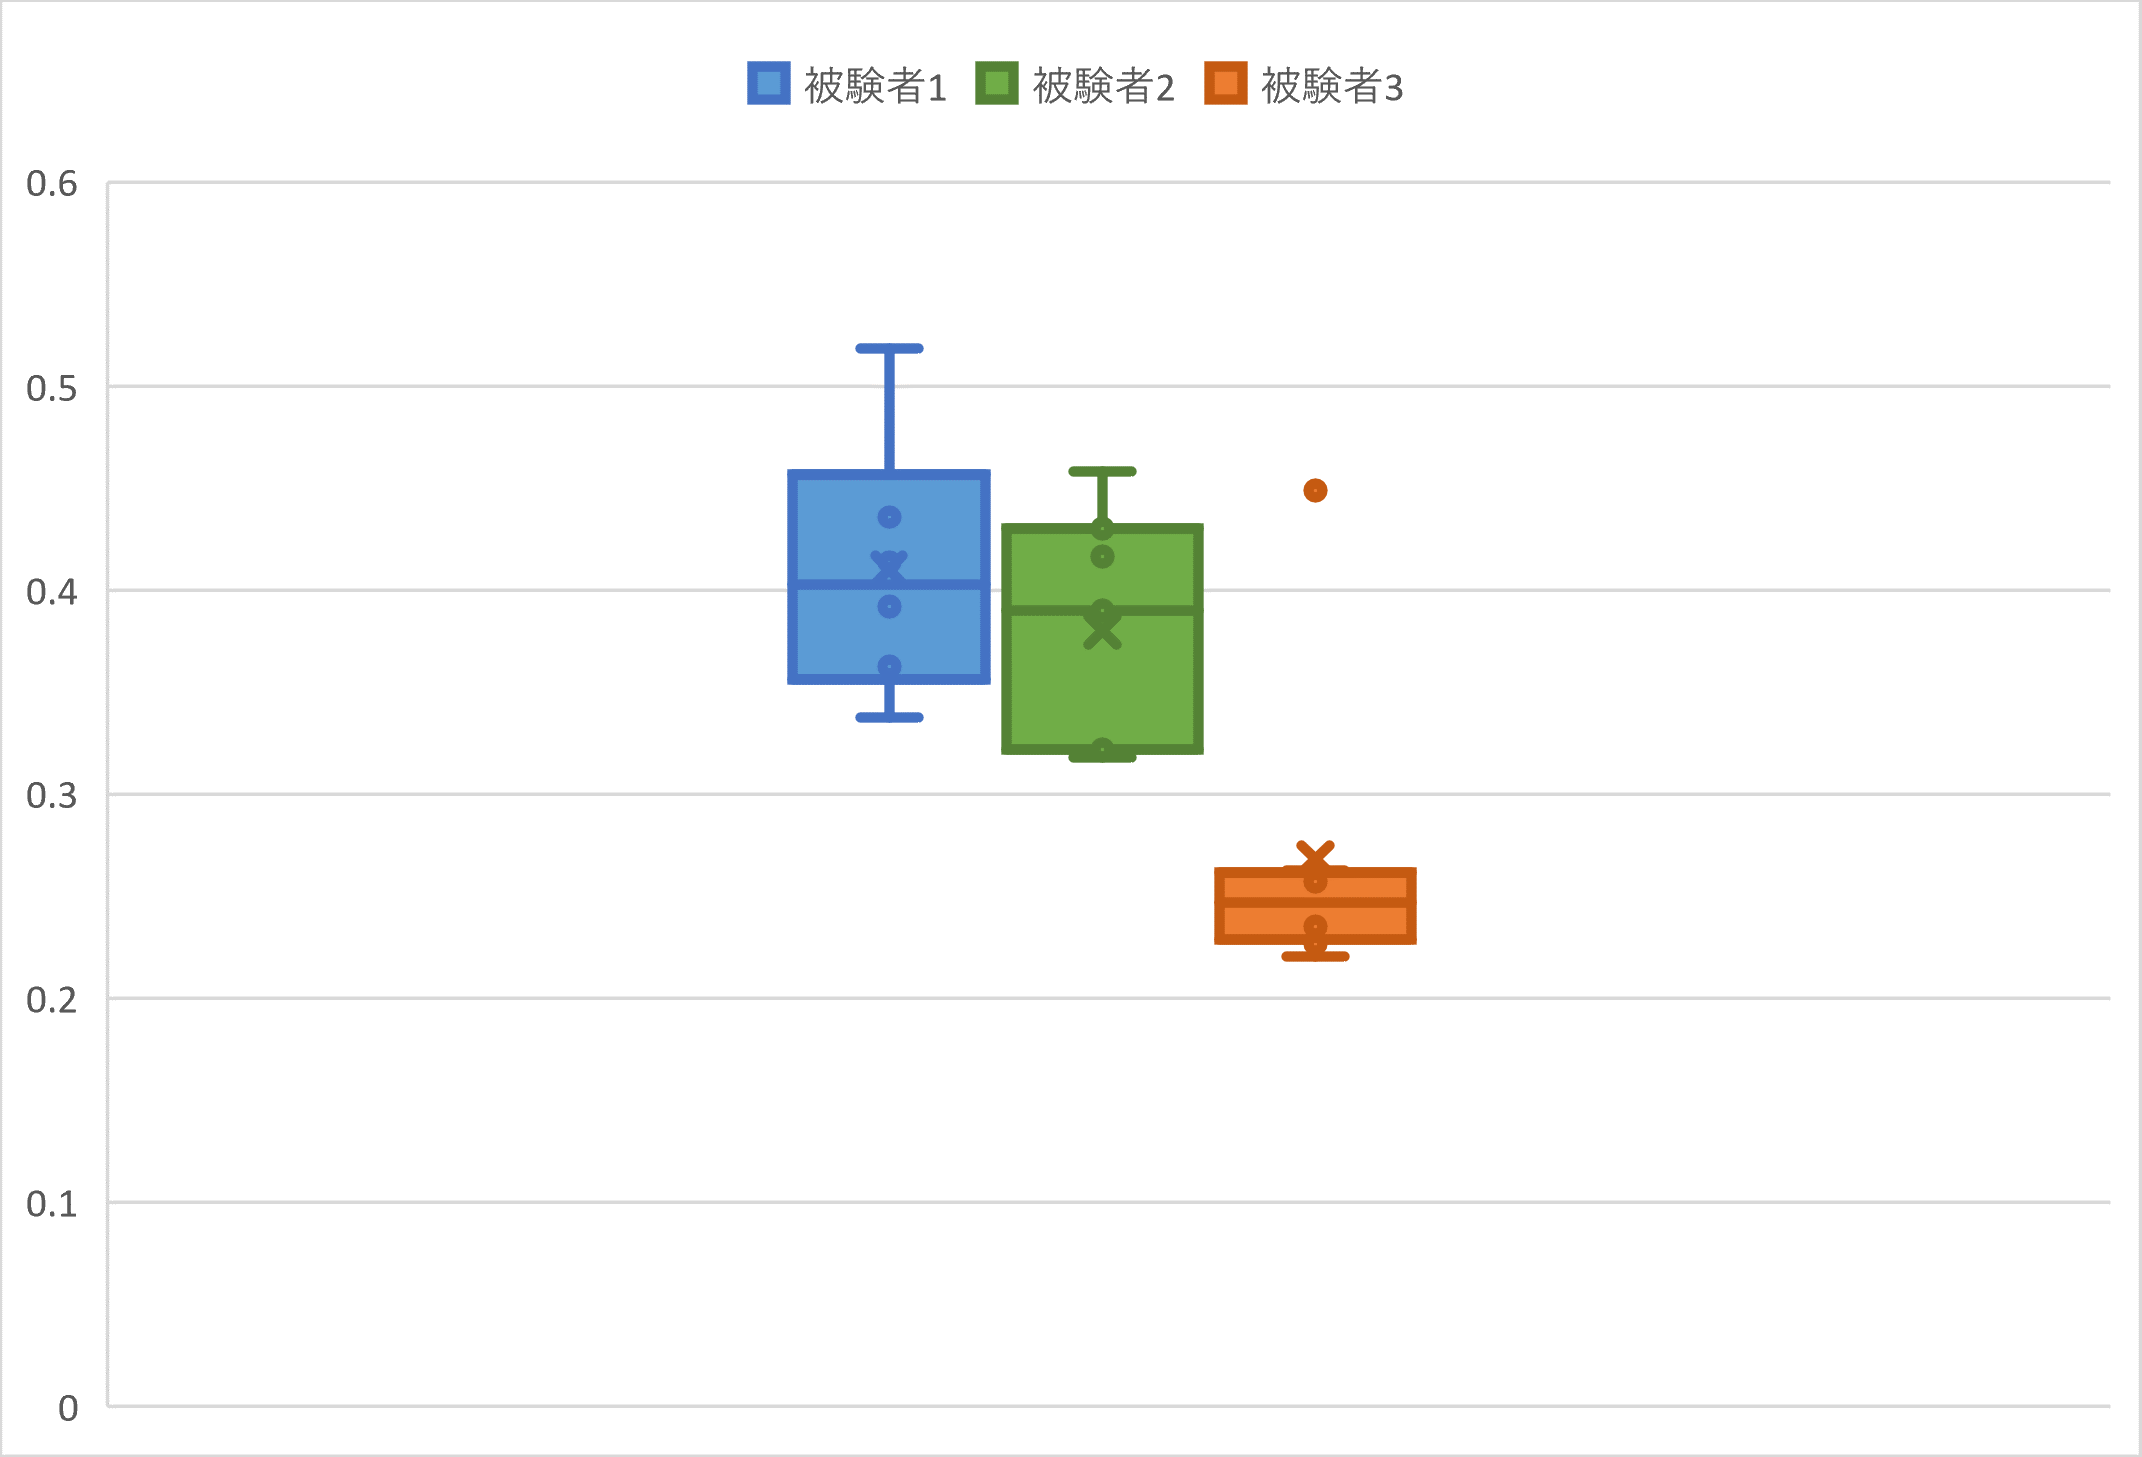
\includegraphics[width=65mm]{hige.png}
 \caption{被験者ごとに色分けした,「ターゲットまでの距離」が80のデータの箱ひげ図}
 \label{hige}
\end{figure}
\noindent


% \subsubsection{棒グラフ}
% 得られたデータのうち,全被験者の「ターゲットまでの距離」ごとの外れ値の数が最も少なかった「ターゲットまでの距離」は,80であった.
% 「ターゲットまでの距離」で昇順に整列したデータのデータ番号を横軸に,「ポインティングが完了するまでの時間」を縦軸に取った棒グラフに作図した結果,図~\ref{bar}のようになった.
% 正規分布か

% % \renewcommand{\figurename}{図}
% \begin{figure}[H]
%  \centering
%    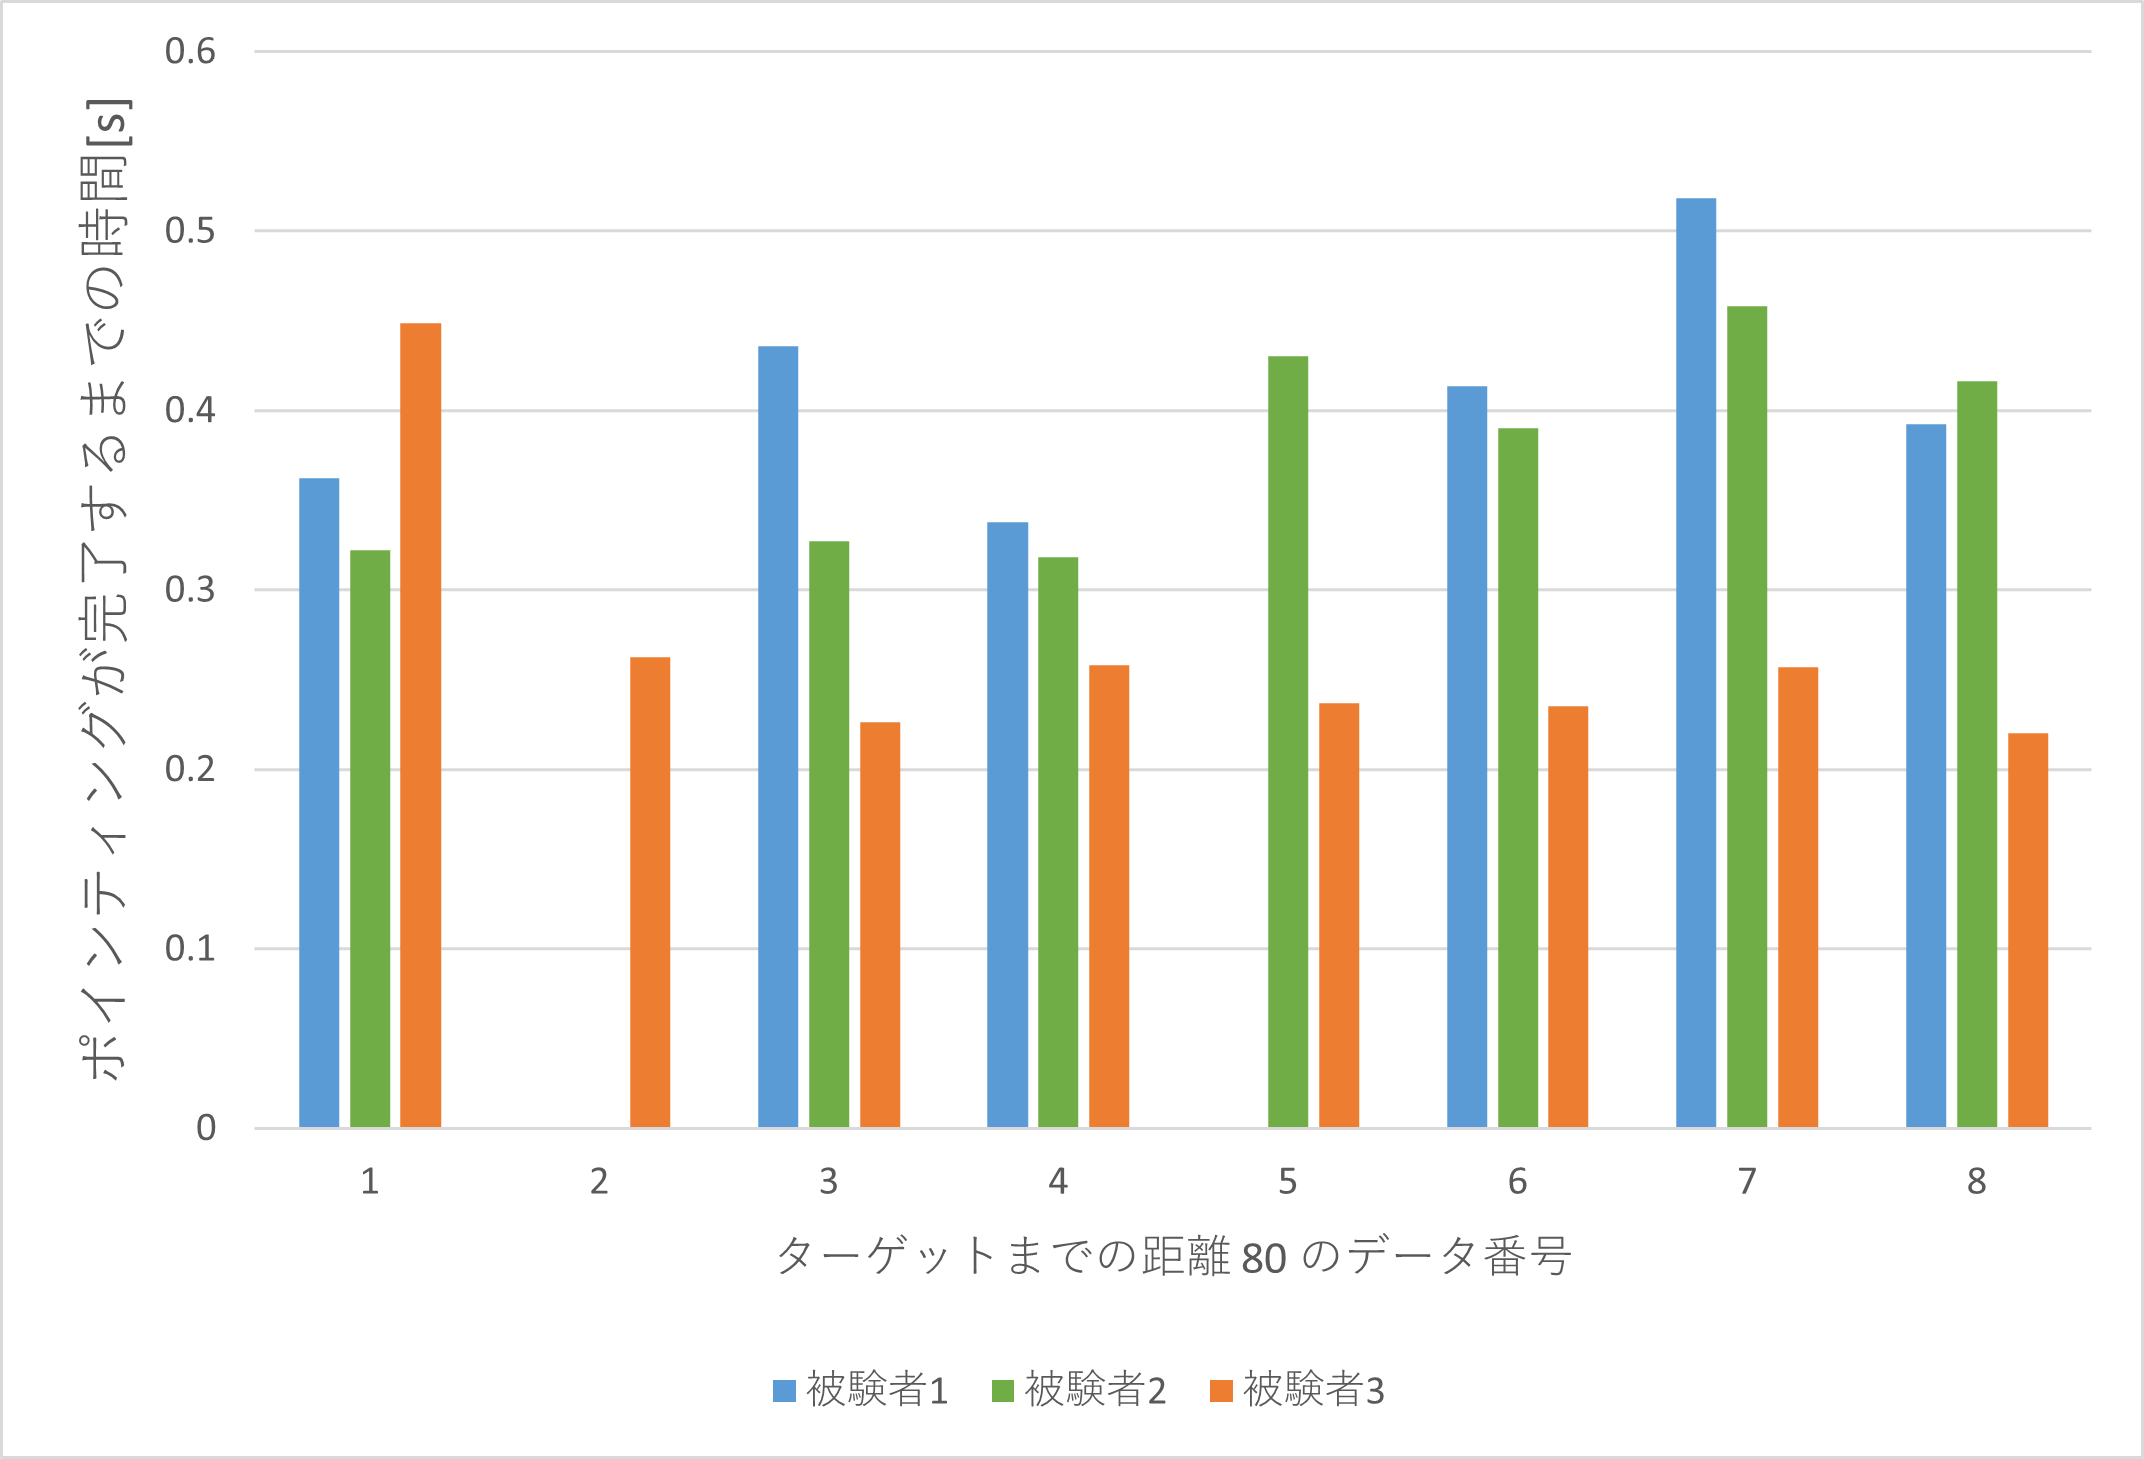
\includegraphics[width=65mm]{bar.png}
%  \caption{被験者ごとに色分けした,「ターゲットまでの距離」が80のデータの棒グラフ}
%  \label{bar}
% \end{figure}
% \noindent

\subsubsection{被験者間の時間のt検定}
最も外れ値の少ない「ターゲットまでの距離」80という同一の条件の下,各被験者の「ポインティングが完了するまでの時間」に有意な差があるかどうかをt検定によって確かめた.
本実験では,各標本の分散はすべて等しいと仮定し,有意水準5\%で両側検定を行った.

検定の結果,被験者1と被験者2との間のp値は約$0.395301 > 0.05$,被験者2と被験者3との間のp値は約$0.006774 < 0.05$,被験者3と被験者1との間のp値は約$0.002827 < 0.05$であった.すなわち,被験者1と被験者2のデータに有意差があるとはいえず,被験者3と被験者1, 2のデータに有意差があるといえた.

したがって,次の分析では被験者1と被験者2はひとつの被験者4のデータとして捉え,被験者3のデータは排除して考えた.
% 有意差がないと解釈していそうで良くない

\subsubsection{ターゲットまでの距離ごとのt検定}
被験者4のデータについて,「ターゲットまでの距離」ごとに「ポインティングが完了するまでの時間」に有意な差が存在するかをt検定によって確かめた.
先ほどと同様,各標本の分散はすべて等しいと仮定し,有意水準5\%で両側検定を行った.

検定の結果,「ターゲットまでの距離」が80と160との間のp値は$0.048623 < 0.05$,160と240との間のp値は$0.256031 > 0.05$,240と320との間のp値は$0.23617 > 0.05$,160と320との間のp値は$0.034407 < 0.05$であった.すなわち,「ターゲットまでの距離」が80と160との間や,160と320との間では「ポインティングが完了するまでの時間」に有意な差があり,「ターゲットまでの距離」が160と240との間や240と320との間では「ポインティングが完了するまでの時間」に有意な差があるとはいえない結果であった.

つまり,「ターゲットまでの距離」がかなり近い時や,差が大きいときには「ポインティングが完了するまでの時間」に有意な差があったといえる.


%%%%%%%%%%%%%%%%%%%%%%%%%%%%%%%%%%%%%%%%%%%%%%%%%%%%%%%%%%%%%%%%%%%%%%%%%%%%%%%%

\section{議論}
散布図を用いた近似曲線の傾きからもt検定の結果からも,仮説「ターゲットまでの距離が遠い場合,ポインティングが完了するまでの時間は長い」は正しいと言えそうである.サンプル数の取り方を工夫し,数を増やせば,より強い仮説の実証が可能であると考える.
% 最初の1回目の試行は除外すべきだった


\begin{comment}
\subsection{実行環境}
\subsubsection{java}
\begin{itemize}
\item javac 11.0.7
\item java 11.0.7 2020-04-14 LTS
\item Java(TM) SE Runtime Environment 18.9 (build 11.0.7+8-LTS)
\item Java HotSpot(TM) 64-Bit Server VM 18.9 (build 11.0.7+8-LTS, mixed mode)
\end{itemize}

\subsubsection{ターミナル}
\begin{itemize}
\item cmd.exe
\begin{itemize}
\item Microsoft Windows [Version 10.0.18363.836]上で実行
\end{itemize}
\end{itemize}

\section{設問}
\subsection{設問1}
\begin{quotation}
【本文】\footnote{【氏名】先生の講義,【講義名】の資料「【資料名】」【ページ数】ページ,$<$ \url{【URL】} $>$ (2020年01月17日アクセス) より抜粋}

【本文】\footnote{芝浦工業大学の学生および教職員向けポータルサイトScombの課題提出ページ「【ページ名】」,$<$ \url{【URL】} $>$ (2020年01月17日アクセス) より抜粋} 
\end{quotation}

\section{目ターゲット}
\subsection{研究の背景}
【本文】

\subsection{研究の目ターゲット}
【本文】

\section{方法}
\subsection{対象}
【本文】
\subsection{装置}
【本文】
\subsection{ソフトウェア}
【本文】
\subsection{ソースプログラム}
\subsubsection{ソースコード}
\setcounter{lstlisting}{4}
\renewcommand{\lstlistingname}{ソースコード}
\begin{lstlisting}[caption = 【ファイル名】, label=【参照名】]
【ソースコード】
\end{lstlisting}

\setcounter{lstlisting}{2}
\renewcommand{\lstlistingname}{実行結果}
\subsubsection{実行結果}
\setcounter{lstlisting}{0}
\renewcommand{\lstlistingname}{実行結果}
\begin{lstlisting}[caption = 【ファイル名】 \quad 【ファイル名】, label = 【参照名】]
\end{lstlisting}

\subsection{手続き}
【本文】

\section{仮説}
【本文】

\section{結果}
【本文】

\section{考察}
\subsection{仮説の吟味}
【本文】
\subsection{その他の考察}
【本文】

\section{結論}
【本文】
~\cite{【サイトの参照名】}.

% \renewcommand{\figurename}{図4-}
\begin{figure}[H]
 \centering
   \includegraphics[width=65mm]{figures/Sample.png}
 \caption{【キャプション名】}
 \label{【ラベル名】}
\end{figure}
\noindent

\end{comment}

%%%%%%%%%%%%%%%%%%%%%%%%%%%%%%%%%%%%%%%%%%%%%%%%%%%%%%%%%%%%%%%%%%%%%%%%%%%%%%%%

\begin{thebibliography}{99}

% F12 -> alert(document.lastModified); でサイトの更新日がわかる
\bibitem{pointing_device_bib}
日本大百科全書(ニッポニカ)(2020)
「ポインティングデバイス」,
\verb|<| \url{https://japanknowledge.com/lib/display/?lid=1001050309103} \verb|>|
2020年10月25日アクセス.

\bibitem{unity_bib}
Unity Technologies (2020)
「Unity のプラットフォーム」,
\verb|<| \url{https://unity.com/ja/products/unity-platform} \verb|>|
2020年10月25日アクセス.

\bibitem{zihou_bib}
OtoLogic (2020)
「効果音>カウントダウン」,
\verb|<| \url{https://otologic.jp/free/se/countdown01.html} \verb|>|
2020年10月25日アクセス.

\bibitem{click_bib}
OtoLogic (2020)
「効果音>PC・マウス」,
\verb|<| \url{https://otologic.jp/free/se/pc-mouse01.html} \verb|>|
2020年10月25日アクセス.
\end{thebibliography}

\begin{comment}
メモ
\end{comment}

\end{multicols}

\end{document}
